\documentclass[11pt,a4paper]{article}
\usepackage[utf8]{inputenc}
\usepackage[T1]{fontenc}
%\usepackage{gentium}
\usepackage{mathptmx} % Use Times Font

\usepackage{graphicx} % Required for including pictures
\graphicspath{ {Figures} }
\usepackage{hyperref} % Format links for pdf
\usepackage{biblatex}
\addbibresource{references.bib}
\usepackage{booktabs} % Used so that tables generated by pandas
                      % to_latex() work correctly

\frenchspacing % No double spacing between sentences
\usepackage[margin=1in]{geometry}

\usepackage[all]{nowidow} % Tries to remove widows
% \usepackage[protrusion=true,expansion=true]{microtype} % Improves typography, load after fontpackage is selected

\usepackage{lipsum} % Used for inserting dummy 'Lorem ipsum' text into the template
\usepackage{multicol}

\title{Comparing Critics to the General Public: Who is a better predictor of a movie's success?}
\author{Jacob Inwald and Ollie Jones}
\date{}

\begin{document}

\maketitle

    %% INSTRUCTIONS: % % 1. Create your own copy of this Overleaf project. You can
    %either edit your report % using: % % a. Overleaf professional, a collaborative
    %LaTeX editor. You can click % "Copy Project" from the Overleaf menu to create a
    %version where you have % read and write permissions. See the following for
    %documentation: % https://www.overleaf.com/edu/edinburgh and %
    %https://uoe.sharepoint.com/:f:/r/sites/digitalskillsandtraining/Shared%20Docume
    %nts/LaTeX/LaTeX%20for%20Beginners%20using%20Overleaf?csf=1&web=1&e=cPqTI3 % %
    %b. A LaTeX editor on your PC. For this option, you can download the source % of
    %this project as a zip (via the Overleaf menu). % % 2. Please rename this file
    %fds-project-option-1.tex, % fds-project-option-2.tex, or
    %fds-project-option-3.tex, depending on % which project option you are doing.
    %When you submit, please submit % the PDF file with the corresponding name. % %
    %3. Please keep the section and paragraph headings as they % are. You should
    %delete all the text within the headings, e.g. % the text that says "What is the
    %area of this data science % study, and why is it interesting to investigate"
    %and the % bullet points. Keeping the headings makes the report a lot % easier
    %for the markers to read, and making things easy for % markers is always
    %beneficial. % % 4. The word limit for the Overview section is mandatory. For
    %the % other sections word limits are suggested. % % 5. The page limits must be
    %strictly adhered to, and depend on if % you are working individually, in pairs
    %or in threes: % % - Individual: 6 pages % - Pairs: 8 pages % - Threes: 10 pages
    %%

    \section{Overview}
    \paragraph{}
        This report analyses the impact of critics on the success of movies within the
            film industry.
        We carried out this analysis using data from IMDb which provided statistics on
            one thousand movies released between 2006 and 2016.
        A least squares multiple regression model was used to determine which factors
            of a movie can be used to predict their box office success, while another least
            squares multiple regression model was used to determine if critics were able to
            predict success based on a metric which combines the revenue and viewer rating
            of that movie.
        We found that a movie's revenue can be predicted by the number of votes it has
            on IMDb, its runtime and the experience of actors in its leading roles.
        We further found that critics ratings cannot be used to predict the overall
            success of a movie, but can predict how the public will recieve it.


    \section{Introduction}
    % Suggested 400 words

    \paragraph{Context and motivation}
        We explore this dataset using data analytics,

            \paragraph{Previous work} Brief description of any previous work in this area
                (e.g., in the media, or scientific literature or blogs).

        E.g. Recent surveys show that most students prefer final projects to final
            exams \cite{Space2021}.

    \paragraph{Objectives}
        What questions are you setting out to answer?
        We set out to investigate the relationship between various factors and the
            rating or gross revenue of a movie.
        There are are various factors that can come into play affecting the rating a
            movie gets or the success of that movie at box office.
        As such, we will only focus on a few of these factors, looking specifically at:
        Director, Actors, Genre and Runtime.
        We will investigate the effect these factors have on movie reception, and
            attempt to determine which are most impactful to the success of a movie.

    \newpage
    \section{Data}
    % Suggested 300 words

    \paragraph{Data provenance}
        We utilized two movie datasets: an IMDb dataset~\cite{data:IMDb} and
            TMD~\cite{data:TMD} (The Movie Dataset).
        The IMDb dataset contains data about movies made from 2006-2016, while the TMD
            dataset contains data about movies released on or before July 2017.
        Both datasets were obtained from kaggle.com and are shared under the CC0 1.0
            Universal Public Domain Dedication.
        TMD is merged data from TMDb (The Movie DataBase) and grouplens.org, a movie
            ranking site.
        However, we only used the part that was obtained from TMDb.
        It is worth noting that the provenance of the IMDb dataset has been subject to
            controversy as it was scraped from IMDb.com.

    \paragraph{Data description}
        The IMDb movie dataset contains 12 columns with string or floating point
            values. 
        The only column of note is the Genre column, which can only take on 12 distinct values, 
            shown in Table \ref*{tab-IMDb-Movie-Data-Column-Description}.
        A summary of the columns is provided in Table \ref*{tab-IMDb-Movie-Data-Column-Description}.
        \begin{table}[h]
            \centering
            \begin{tabular}{lp{10cm}l}
                \toprule
                Column Name        & Description                                                                & Data Type \\
                \midrule
                Rank               & The rank the movie has in the IMDb database                                & Integer   \\
                Title              & The name of the movie                                                      & String    \\
                Genre              & The genres that apply to the movie, there can be anywhere from 1-3 genres.
                A genre can be any from: Action, Adventure, Sci-Fi, Thriller, Animation,
                    Comedy, Family, Fantasy, Drama, Music, Romance, History, Crime, Western, War,
                    Musical, Sport, Horror, Mystery, Biography.
                                   & Genre                                                                                  \\
                Description        & The description of the movie                                               & String    \\
                Director           & The person who directed the movie                                          & String    \\
                Actors             & The lead roles in the movie                                                & String    \\
                Year               & The year the movie was released                                            & Integer   \\
                Runtime (Minutes)  & The runtime in minutes of the movie                                        & Integer   \\
                Rating             & The mean rating of the movie, taken from IMDb.com                          & Float     \\
                Votes              & The amount of users that voted on a movie to give it that rating           & Integer   \\
                Revenue (Millions) & The gross income the movie made at the US box office                       & Float     \\
                Metascore          & The rating of movie, determined using aggregated weighted Critics scores   & Integer   \\
                \bottomrule
            \end{tabular}
            \caption[short]{The different columns in the IMDb-Movie-Data.csv file}\label{tab-IMDb-Movie-Data-Column-Description}
        \end{table}

        We worked exclusively with the Crew table in TMD, which is a small part of the
            entire database.
        This table contains three columns - Cast, Crew, and ID.
        The Cast and Crew columns are not composed of discrete data points, 
            but rather JSON files representing the entire cast or crew list. 
        As a result, we extracted the data using string parsing methods. 
        A summary of the columns is provided in Table~\ref{tab-Credits-Column-Description}.
        \begin{table}[h]
            \centering
            \begin{tabular}{lp{10cm}l}
                \toprule
                Column Name & Description                                                              & Data Type  \\
                \midrule
                cast        & The cast list of the movie, including all actors who appeared in it.     & .json file \\
                crew        & The entire crew list of the movie. & .json file \\
                id          & The movie id - used in the larger dataset to connect tables together     & Integer    \\
                \bottomrule
            \end{tabular}
            \caption[short]{The different columns in the credits.csv file}\label{tab-Credits-Column-Description}
        \end{table}

    \paragraph{Data processing}
        We used a Python script to parse the TMD dataset and count the number of
            movies each director and actor has been involved in.
        The resulting datasets were saved as CSV files named actor\_counts.csv and
            director\_counts.csv.
        We then merged this data with the original IMDb
            dataset.
        This involved dropping the Description column and replacing the
            Director and Actor columns with Director Exp. and Mean Lead Roles Exp.
        A summary of the new columns is shown in Table
            \ref*{tab-merged-data-column-description}.
        %----------
        \begin{table}[H]
            \centering
            \begin{tabular}{lp{9cm}l}
                \toprule
                Column Name           & Description                                                  & Data Type \\
                \midrule
                Director Exp.        & Amount of movies director has made & Float     \\
                Mean Lead Roles Exp. & Mean amount of movies lead actors have made & Float     \\
                \bottomrule
            \end{tabular}
            \caption[short]{The different columns in the merged data set, 
                            it also shares all the columns described in Tables
                            \ref*{tab-IMDb-Movie-Data-Column-Description}, 
                            except for Director and Actors}\label{tab-merged-data-column-description}
        \end{table}
        %----------
        To check this data was properly normalised we made a histogram plot of all the
            numeric variables, shown in Figure \ref{fig-distribution-of-numeric-variable}.
        As expected, a few variables did not appear to be normally distributed, namely
        Revenue (Millions), Votes, Runtime (Minutes), Director Exp., and Rating.
        \begin{figure}[H]
            \centering
            \begin{subfigure}[b]{0.75\textwidth}
                \centering
                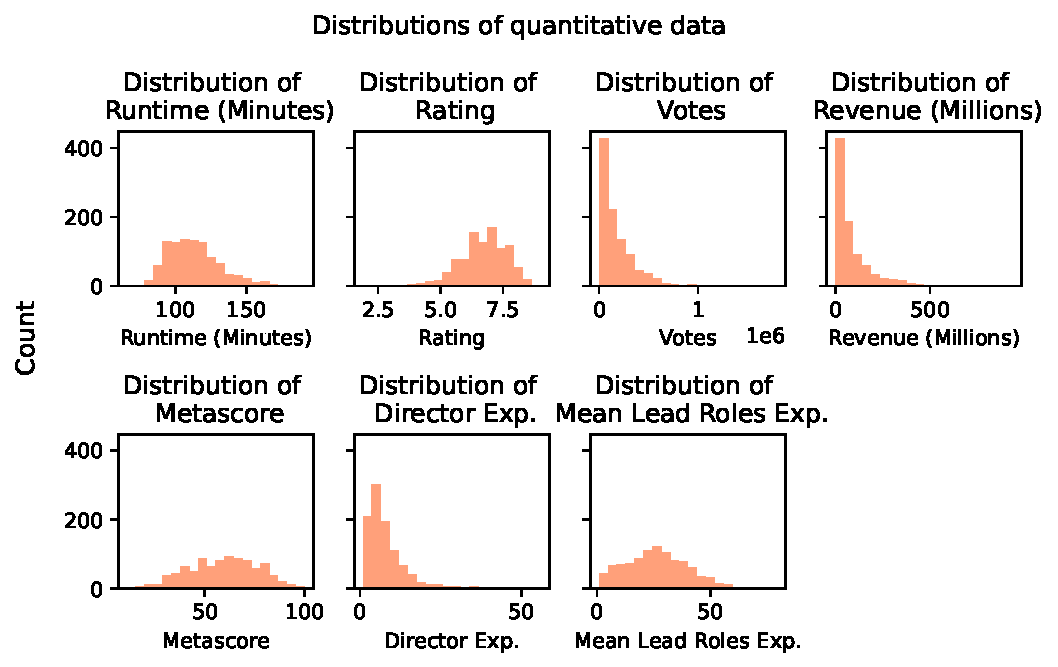
\includegraphics[width=\linewidth]{Final/Distribution of Numeric Variables (No Transformation).pdf}
            \end{subfigure}
            \begin{subfigure}[b]{0.2\textwidth}
                \centering
                \captionsetup{justification=justified,singlelinecheck=false}
                \caption{The distributions of the numeric variables in the merged dataset}\label{fig-distribution-of-numeric-variable}
            \end{subfigure}
            \\
            \begin{subfigure}[b]{0.75\textwidth}
                \centering
                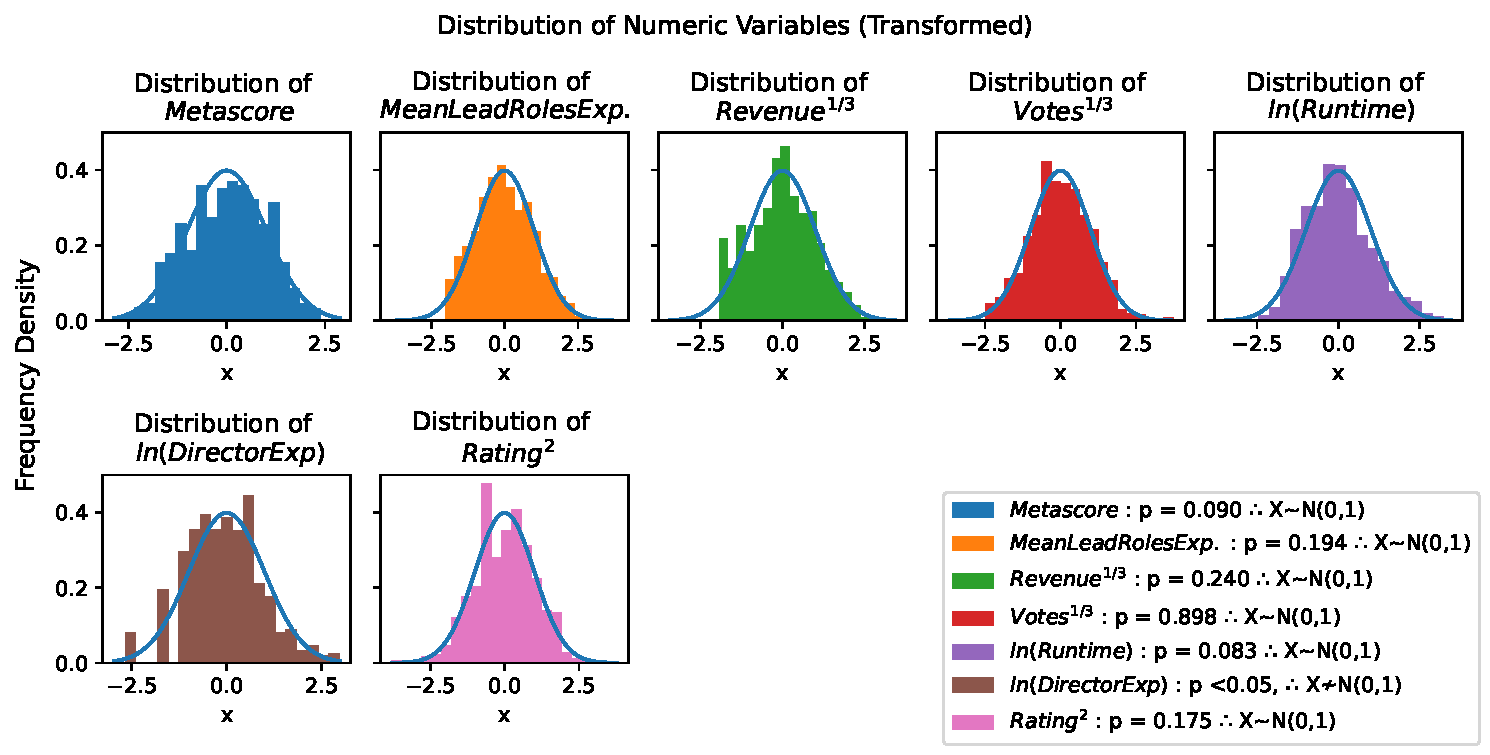
\includegraphics[width=\linewidth]{Final/Distribution of Numeric Variables (Transformed).pdf}
            \end{subfigure}
            \begin{subfigure}[b]{0.2\textwidth}
                \centering
                \captionsetup{justification=justified,singlelinecheck=false}
                \caption{The distributions of the standardised and normalised numeric variables
                        in the merged dataset, the legend has the p-values from testing with 
                        $H_{0}: X \not\sim N(0,1)$. Also shown on the plots is the Gaussian Distribution
                        with the columns mean and standard deviation.}
                \label{fig-transformed-distribution-of-numeric-variable}
            \end{subfigure}
            \caption{Distribution of Numeric Variables in the Merged Dataset}
            \label{fig-numeric-variable-distribution}
        \end{figure}
                  
        Figure \ref*{fig-distribution-of-numeric-variable} shows that Revenue (Millions) and Votes are
        severely right-skewed, implying an exponential distribution. Runtime
        (Minutes) and Director Exp. appear to be less severely right-skewed,
        implying a lognormal distribution. Rating seems to be left-skewed. The
        transformations that give the best approximations to a normal
        distribution are cube root transform for Revenue (Millions) and Votes,
        log transform for Runtime (Minutes) and Director Exp., and square
        transform for Rating.
        
        Figure \ref*{fig-transformed-distribution-of-numeric-variable} shows the
        standarised and normalised numeric variables. The legend contains the p-values
        from the Kolmogorov-Smirnov normality test \cite*{KStest}, which was used to
        test the data against the null hypothesis $H_{0}: X \not\sim N(0,1)$. It is
        worth noting that the Director Exp. column failed the test. Despite this, the histogram follows a
        normal distribution curve and there appears to be missing data, providing convincing evidence that ln(Director Exp.)
        has a normal distribution. Ultimately, these transformations helped to normalize
        the dataset and improve its suitability for further analysis.

        To make use of the Genre column, one-hot encoding was used.
        We added a column for each Genre and set each entry to 1 if the corresponding
            movie fit that genre and 0 otherwise.
        Genres with less than 100 movies made were excluded to ensure a large enough
            sample size was present, such that we could draw meaningful conclusions.

    \newpage
    \newpage
\section{Exploration and Analysis}
    \subsection{What makes a movie successful?}
        \begin{multicols}{2}
            % We would like you to explore what makes a movie popular and/or successful.
            \paragraph{}
                In order to ascertain which factors are most influential in determining the
                    success of a movie, it is necessary to first define what constitutes success.
                For the purpose of this analysis, success is defined as the movie's revenue.
                By examining the correlations between the movie's revenue and other factors, we
                    can gain insight into which factors have the greatest impact on the success of
                    a movie.
                These correlations are visualised in Figure~\ref{fig-heatmap}.

                \begin{figure}[H]
                    \centering
                    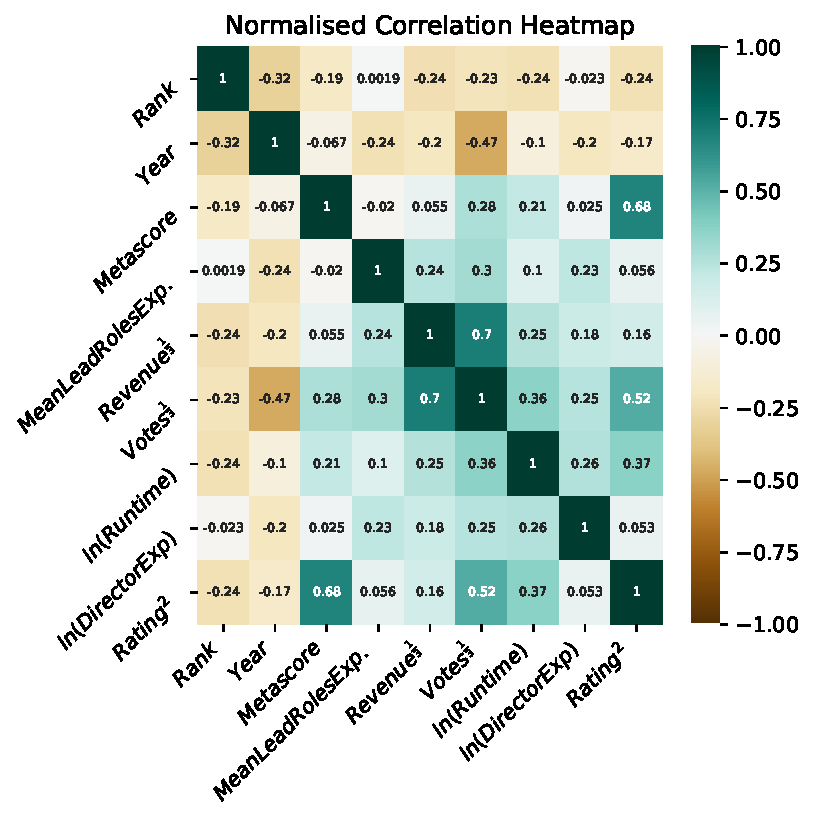
\includegraphics[width=\linewidth]{Final/Normalised Correlation Heatmap.pdf}
                    \caption{
                        A heatmap illustrating the strength of correlations (using PMCC) between various normalised
                        variables from the IMDb dataset~\cite{data:IMDb} and the TMD
                        data~\cite{data:TMD}.
                    }\label{fig-heatmap}
                \end{figure}

            \paragraph{}
                Figure~\ref{fig-heatmap} reveals a strong positive correlation (0.7) between a
                    movie's revenue and the number of votes it receives on IMDb, suggesting that
                    the more votes a movie receives, the higher its revenue is likely to be.
                Additionally, the heatmap shows moderate positive correlations between the
                    movie's revenue and its runtime (0.25) and between the movie's revenue and the
                    experience of the actors in lead roles (0.24), indicating that longer runtimes
                    and more experienced actors may be associated with higher revenues.
                In contrast, there is a moderate negative correlation between a movie's revenue
                    and its rank on IMDb (-0.24), suggesting that higher ranks on IMDb do not
                    necessarily translate to higher revenues.
                These four correlations are shown in more detail in
                    Figure~\ref{fig-revenue-factors}.

                \begin{figure}[H]
                    \centering
                    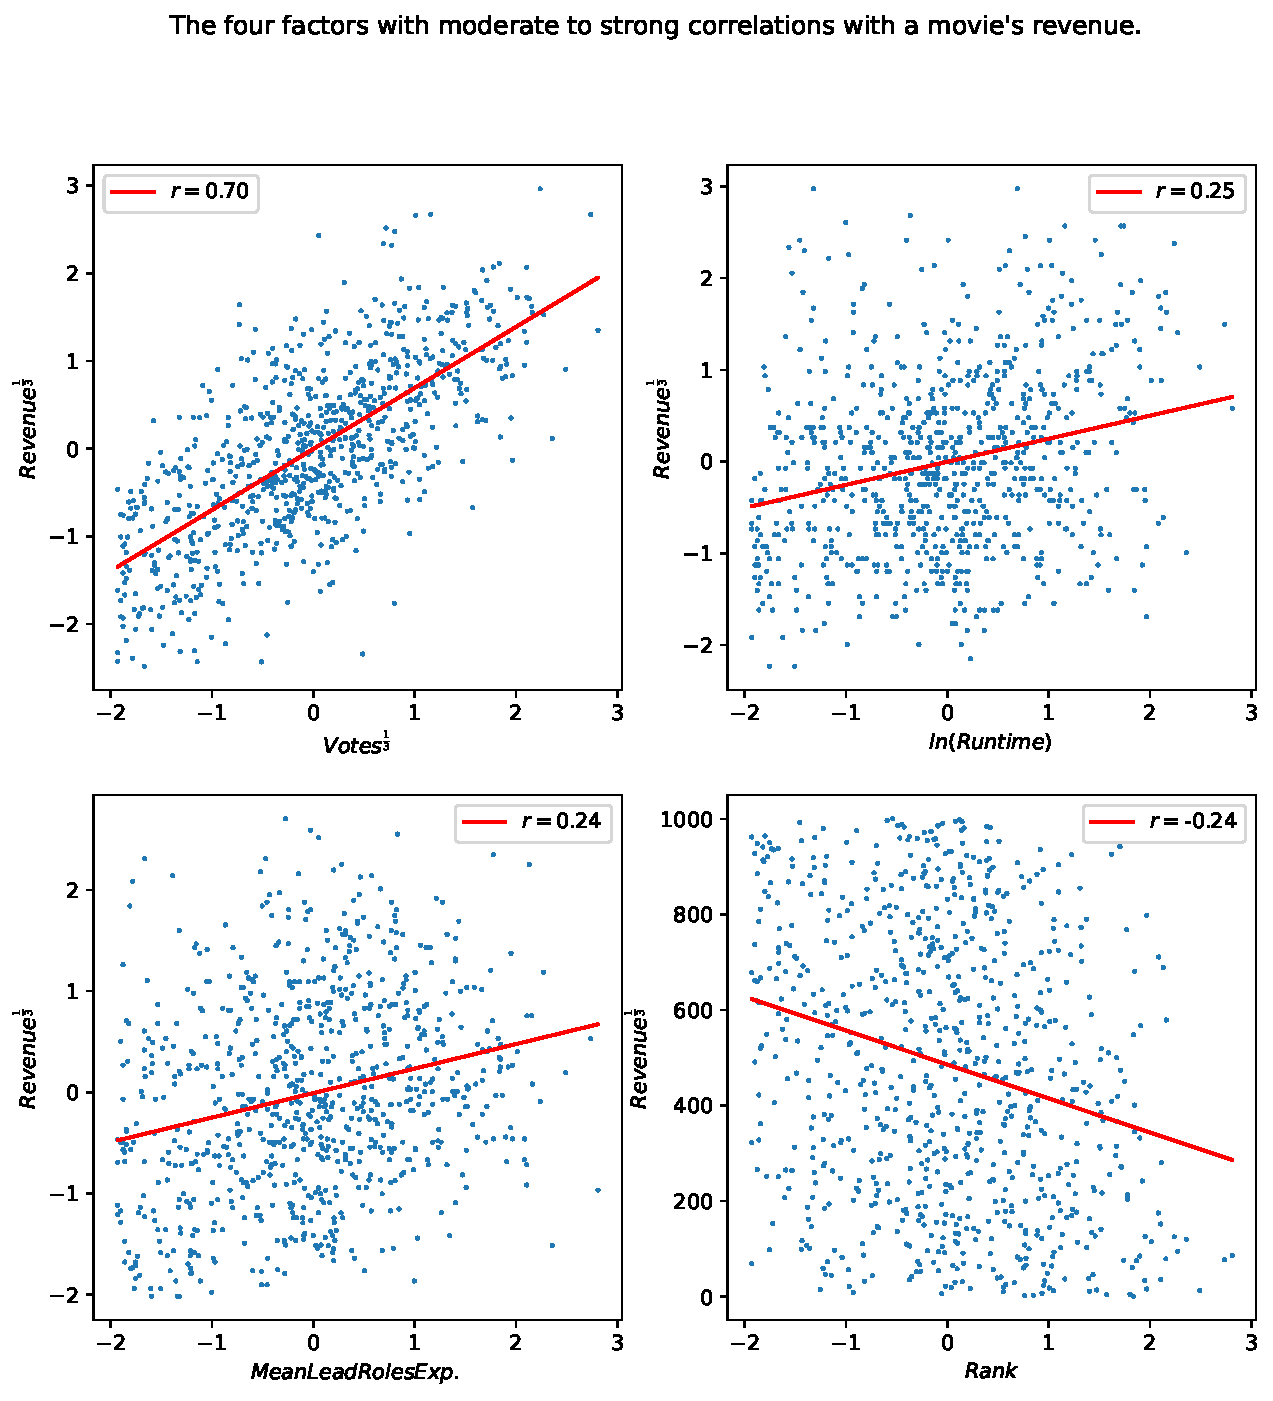
\includegraphics[width=\linewidth]{Final/Revenue Factors.pdf}
                    \caption{
                        Scatter plots showing the relationships between a movie's revenue and the four
                        factors with moderate or strong correlations.
                    }\label{fig-revenue-factors}
                \end{figure}
        \end{multicols}

    \subsection{The relationship between a movie's ranked position and its number of votes}
        \begin{multicols}{2}
            % We would also like you to visualise the distribution of ranked position and
            % number of votes, and comment on the relationship between them.
            \paragraph{}
                IMDb's system for ranking movies is connected to the votes cast by viewers.
                The statistical distributions of the ranks and the votes are show in
                    Figure~\ref{fig-rank-vote-dist} and the correlation between these two varaibles
                    is shown in Figure~\ref{fig-rank-vote-corr}.
                This data suggests that lower ranked movies have more votes, which implies that
                    people give lower ratings more often than they give higher ones.

                \begin{figure}[H]
                    \centering
                    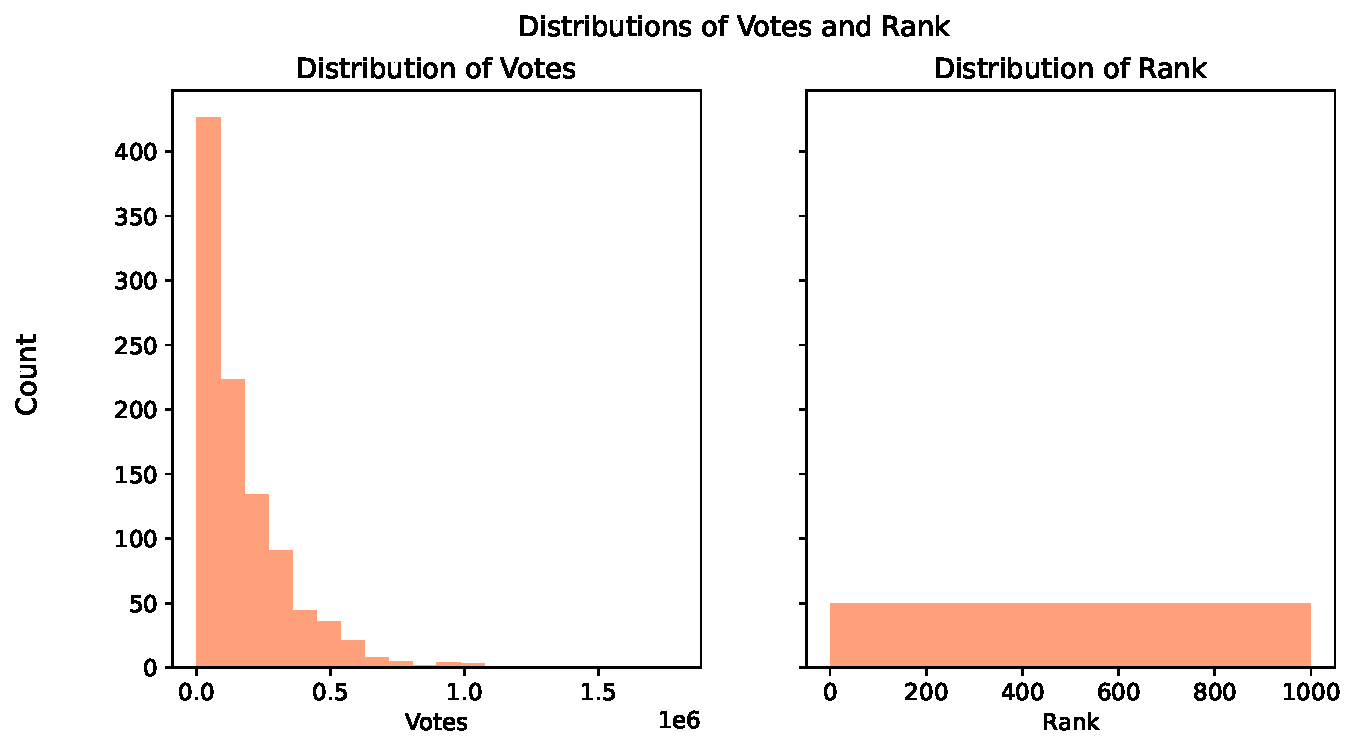
\includegraphics[width=\linewidth]{Final/Distributions of Votes and Rank.pdf}
                    \caption{}\label{fig-rank-vote-dist}
                \end{figure}

                \begin{figure}[H]
                    \centering
                    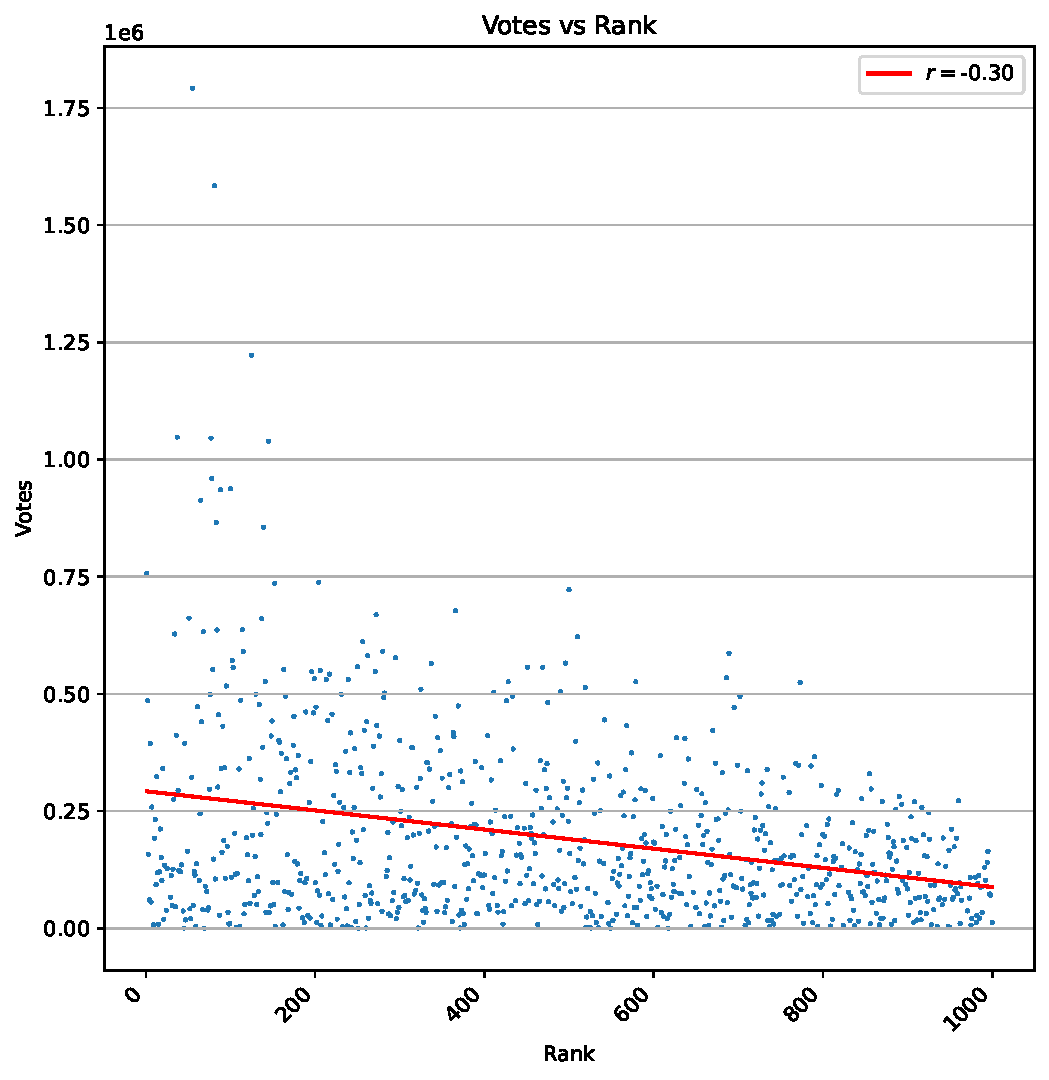
\includegraphics[width=\linewidth]{Final/Votes vs Rank.pdf}
                    \caption{}\label{fig-rank-vote-corr}
                \end{figure}
        \end{multicols}

    \subsection*{}
        \paragraph{}

    % Suggested 500 words for individual report; proportionately longer for group
    % projects).
    % Revenue Multiple Regression
    \subsection{What factors can predict box office success?}
    % We would like you to explore what makes a movie popular and/or successful.
        \paragraph{}
        In order to further analyze the correlations between the various movie details
        and the revenue they generated, we created a multiple regression model using the
        normalized data we collected. 
        The target variable was the normalised revenue, with the rest of the dataset as the 
            predictor variables, excluding Genre and Title.
        $Votes^\frac{1}{3}$ was excluded as it is causally linked to Revenue; the more votes, the more people bought movie tickets. 
        The model uses Ordinary Least Squares regression and a constant column has been added to show y-intercept.
        The summary results are provided in Table \ref{tab-revenue-ols-summary}.
        \begin{table}[H]
            \begin{center}
                \begin{tabular}{lclc}
                    \toprule
                    \textbf{Dep. Variable:}           &  $Revenue^{\frac{1}{3}}$   & \textbf{  R-squared:         } &     0.404   \\
                    \textbf{Model:}                   &       OLS        & \textbf{  Adj. R-squared:    } &     0.393   \\
                    \textbf{Method:}                  &  Least Squares   & \textbf{  F-statistic:       } &     36.60   \\
                    \textbf{No. Observations:}        &         826      & \textbf{  Prob (F-statistic):} &  1.35e-80   \\
                    \textbf{Df Residuals:}            &         810      & \textbf{Df Model:}             &       15  \\
                    \bottomrule
                \end{tabular}
                \begin{tabular}{lcccccc}
                                                    & \textbf{coef} & \textbf{std err} & \textbf{t} & \textbf{P$> |$t$|$} & \textbf{[0.025} & \textbf{0.975]}  \\
                    \midrule
                    \textbf{$const$}                &     114.0116  &       19.712     &     5.784  &         0.000        &       75.319    &      152.705     \\
                    \textbf{$Rank$}                 &      -0.0006  &        0.000     &    -5.654  &         0.000        &       -0.001    &       -0.000     \\
                    \textbf{$Year$}                 &      -0.0565  &        0.010     &    -5.770  &         0.000        &       -0.076    &       -0.037     \\
                    \textbf{$Metascore$}            &       0.0416  &        0.038     &     1.093  &         0.275        &       -0.033    &        0.116     \\
                    \textbf{$Mean Lead Roles Exp.$} &       0.1125  &        0.030     &     3.793  &         0.000        &        0.054    &        0.171     \\
                    \textbf{$ln(Runtime)$}          &       0.1705  &        0.033     &     5.203  &         0.000        &        0.106    &        0.235     \\
                    \textbf{$ln(Director Exp)$}     &       0.0507  &        0.029     &     1.756  &         0.079        &       -0.006    &        0.107     \\
                    \textbf{$Rating^2$}             &       0.0816  &        0.041     &     2.013  &         0.044        &        0.002    &        0.161     \\
                    \textbf{$Action$}               &       0.1824  &        0.070     &     2.598  &         0.010        &        0.045    &        0.320     \\
                    \textbf{$Adventure$}            &       0.4765  &        0.074     &     6.452  &         0.000        &        0.332    &        0.621     \\
                    \textbf{$Sci-Fi$}               &       0.0318  &        0.087     &     0.364  &         0.716        &       -0.140    &        0.203     \\
                    \textbf{$Thriller$}             &      -0.0395  &        0.078     &    -0.504  &         0.615        &       -0.193    &        0.114     \\
                    \textbf{$Comedy$}               &       0.1145  &        0.072     &     1.599  &         0.110        &       -0.026    &        0.255     \\
                    \textbf{$Drama$}                &      -0.5579  &        0.071     &    -7.877  &         0.000        &       -0.697    &       -0.419     \\
                    \textbf{$Romance$}              &      -0.0243  &        0.084     &    -0.288  &         0.773        &       -0.190    &        0.141     \\
                    \textbf{$Crime$}                &      -0.0545  &        0.082     &    -0.664  &         0.507        &       -0.216    &        0.107     \\
                    \bottomrule
                \end{tabular}
            \end{center}
            \caption[short]{Multiple regression results with $Revenue^{\frac{1}{3}}$ as the dependent variable
                            and the normalised data as the independent variable. The OLS approach was used to
                            find the best fit. The residuals for this model are shown in 
                            fig \ref{fig-revenue-ols-residuals}}\label{tab-revenue-ols-summary}
        \end{table}
        This model performs respectably, explaining about  40\% of the variance in box office success.
        It is also statistically significant ($R^2=0.404, F(15,810)=36.6, p<0.05$).
        The results indicate a well performing model, and as such we can postulate 
            that at least some of these factors are impactful on the box office success a movie has.

        % Director vs Actor for selling tickets
        The results suggest that box office sales can be predicted by lead actor experience ($\beta=0.113, \sigma=0.030, p<0.05$),
            but cannot be predicted by director experience ($\beta=0.051, \sigma=0.030, p>0.05$).
        Previous research has shown that movie advertising tends to be focussed around the actors 
            present more than the director of the movie\cite{elberse2007power}.
        Examples of this are present in adverts like movie posters - actor faces feature front and 
            center while directors are listed in name only.
        Actors who have been in many movies are more recognisable, meaning potential consumers
            will be more likely to invest money in seeing a movie they are part of.

        % Meta score vs Rating
        The results also suggest that box office sales can't be predicted by critics (Metascore) 
            ($\beta=0.042, \sigma=0.038, p>0.05$), but can be predicted by user rating.
            ($\beta=0.082, \sigma=0.041, p<0.05$).
        It is reasonable to assume both would have similar quality as predictor variables - they 
            correlate strongly (see fig \ref{fig-heatmap}).
        As such, the difference in quality is surprising.
        This difference could be due to movies appearing in the box office for only a short period.
        Revenue is only calculated during this period, a period of time where consumers may 
            rely on friends rather than a critics review, as those often come out later.
        With this in mind, it is reasonable to say that critics do not appear to be able to predict the likelihood
            of a movie becoming a blockbuster.
        
        % Genre notes
        Finally, there are some interesting notes about the impact of genre has on the box office success of a movie.
        Adventure seems to have the biggest positive impact on box office success ($\beta=0.477,\sigma=0.074,p<0.05$).
        Dramas appear to have the largest negative impact on box office success ($\beta=-0.558,\sigma=0.071,p<0.05$).
    \subsection{Can critics truly predict movie success?}
        % We would like you to explore what makes a movie popular and/or successful.
        \paragraph{}
        % Success metric definition
        To analyze the effect critics had on predicting general success of a movie, we define
            a metric of success, $Success = \frac{Revenue^\frac{1}{3} + Rating^2}{2}$.
        We chose this metric as Revenue and Rating are both measures of movie success,
            and Figure \ref{fig-heatmap} shows that they are not strongly correlated.
        This means they describe independent aspects of success, and therefore the mean of both
            will better encapsulate the true success of a movie.
        We refer to this metric as success from now on.
        
        To investigate the ability for critics to predict movie success, we present a multiple regression model,
            with the target variable being the success metric. 
        We used the rest of the normalised dataset for predictor variables, excluding the $Revenue^\frac{1}{3}$, $Rating^2$,
            Genre and Title columns.
        Genre and Title were excluded as they are not quantative data and $Revenue^\frac{1}{3}$ and $Rating^2$ were excluded
            as they are causally  linked to the success metric.
        We use the same approach as in Table \ref{tab-revenue-ols-summary}, with a constant column and using OLS.
        The summary results are provided in Table \ref{tab-success-ols-summary}.
        \begin{table}[H]
            \begin{center}
                \begin{tabular}{lclc}
                    \toprule
                    \textbf{Dep. Variable:}           &     Success      & \textbf{  R-squared:         } &     0.758   \\
                    \textbf{Model:}                   &       OLS        & \textbf{  Adj. R-squared:    } &     0.753   \\
                    \textbf{Method:}                  &  Least Squares   & \textbf{  F-statistic:       } &     169.1   \\
                    \textbf{No. Observations:}        &         826      & \textbf{  Prob (F-statistic):} & 2.67e-237   \\
                    \textbf{Df Residuals:}            &         810      & \textbf{Df Model:}             &       14     \\
                    \bottomrule
                \end{tabular}
                \begin{tabular}{lcccccc}
                                                    & \textbf{coef} & \textbf{std err} & \textbf{t} & \textbf{P$> |$t$|$} & \textbf{[0.025} & \textbf{0.975]}  \\
                    \midrule
                    \textbf{$const$}                &     -49.4262  &       10.871     &    -4.547  &         0.000        &      -70.765    &      -28.087     \\
                    \textbf{$Rank$}                 &      -0.0001  &     5.42e-05     &    -2.173  &         0.030        &       -0.000    &    -1.14e-05     \\
                    \textbf{$Year$}                 &       0.0246  &        0.005     &     4.560  &         0.000        &        0.014    &        0.035     \\
                    \textbf{$Metascore$}            &       0.1858  &        0.015     &    12.006  &         0.000        &        0.155    &        0.216     \\
                    \textbf{$Mean Lead Roles Exp.$} &      -0.0003  &        0.015     &    -0.022  &         0.983        &       -0.029    &        0.028     \\
                    \textbf{$Votes^{\frac{1}{3}}$}  &       0.5669  &        0.020     &    28.674  &         0.000        &        0.528    &        0.606     \\
                    \textbf{$ln(Runtime)$}          &       0.0820  &        0.016     &     5.185  &         0.000        &        0.051    &        0.113     \\
                    \textbf{$ln(Director Exp)$}     &      -0.0318  &        0.014     &    -2.286  &         0.023        &       -0.059    &       -0.004     \\
                    \textbf{$Action$}               &      -0.0532  &        0.034     &    -1.561  &         0.119        &       -0.120    &        0.014     \\
                    \textbf{$Adventure$}            &       0.1279  &        0.036     &     3.554  &         0.000        &        0.057    &        0.199     \\
                    \textbf{$Sci-Fi$}               &      -0.2271  &        0.043     &    -5.300  &         0.000        &       -0.311    &       -0.143     \\
                    \textbf{$Thriller$}             &      -0.0610  &        0.038     &    -1.610  &         0.108        &       -0.135    &        0.013     \\
                    \textbf{$Comedy$}               &       0.0376  &        0.035     &     1.087  &         0.277        &       -0.030    &        0.106     \\
                    \textbf{$Drama$}                &      -0.0391  &        0.035     &    -1.133  &         0.258        &       -0.107    &        0.029     \\
                    \textbf{$Romance$}              &      -0.0858  &        0.041     &    -2.103  &         0.036        &       -0.166    &       -0.006     \\
                    \textbf{$Crime$}                &      -0.0795  &        0.040     &    -2.003  &         0.046        &       -0.157    &       -0.002     \\
                    \bottomrule
                \end{tabular}
            \end{center}
        \caption[short]{Multiple regression results with $Revenue^{\frac{1}{3}}$ as the dependent variable
                        and the normalised data as the independent variable. The OLS approach was used to
                        find the best fit. The residuals for this model are shown in 
                        fig \ref{fig-success-ols-residuals}}\label{tab-success-ols-summary}
        \end{table}
    This model performs very well, explaining about 75\% of the variance in user ratings.
        It is also statistically significant ($R^2=0.758, F(14,810)=169, p<0.05$).
    The results indicates a well performing model, and as such we can postulate 
        that at least some of these factors are impactful on the success a movie has.

    % Metascore analysis
    The results show that movie success can be well predicted by Metascore ($\beta=0.186, \sigma=0.015, p<0.05$).
    This compares to how it is not a good predictor of Revenue (see Table \ref{tab-revenue-ols-summary}).
    This difference shows that while critics can't predict the box office success, they can predict the 
        overall success of the movie.
    Metascore is one of the key predictors in this model - with the third largest absolute coefficient - 
        demonstrating that critics are important when it comes to predicting the success of a movie.
    This idea is supported by the PPMCC that Metascore has with the Success metric ($R^2=0.48$).
    This is a relatively strong correlation, suggesting that critics can discern potentially successful movies.
    
    % Constant
    Another observation is the constants coefficient is negative ($\beta=-49.4,\sigma=10.9,p<0.05$).
    This means that the average movie tends to not be very successful, which is inline with research that
        most movies do not succeed, with only a few actually garnering actual success \cite{walls2005modelling}.

    % Genre notes
    Finally, there are some interesting notes about the impact of genre has on the box office success of a movie.
    Adventure seems to have the biggest positive impact on success ($\beta=0.128,\sigma=0.036,p<0.05$).
    Sci-Fi appears to have the largest negative impact on success ($\beta=-0.223,\sigma=0.043,p<0.05$).

\begin{figure}[H]
    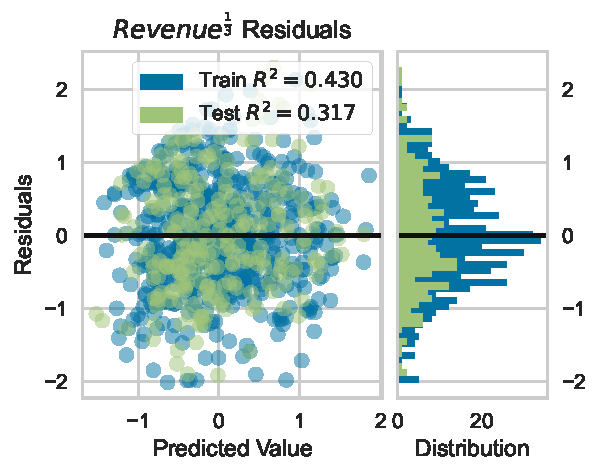
\includegraphics[width=\linewidth]{/Final/Revenue OLS Residuals.pdf}
    \caption[short]{title}\label{fig-revenue-ols-residuals}
\end{figure}

\begin{figure}[H]
    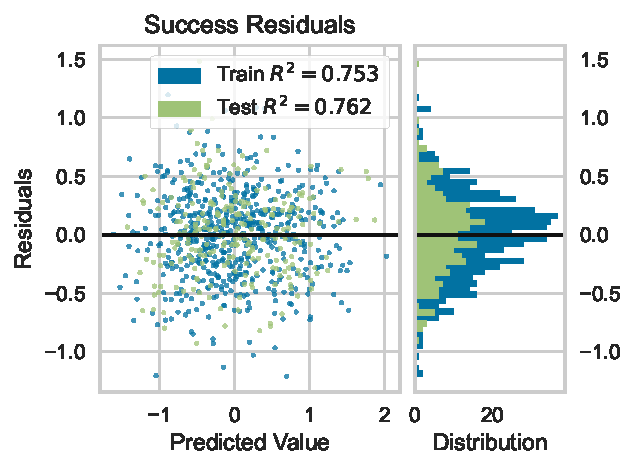
\includegraphics[width=\linewidth]{/Final/Success OLS Residuals.pdf}
    \caption[short]{title}\label{fig-success-ols-residuals}
\end{figure}

    \section{Discussion and Conclusions}
    % Suggested 400 words.

    \paragraph{Summary of findings}

    \paragraph{Evaluation of own work: strengths and limitations}

    \paragraph{Comparison with any other related work}
        E.g. ``Anscombe has also demonstrated that many patterns of data can have the
            same correlation coefficient'' \cite{anscombe1973graphs}.

        Wikipedia can also be cited but it is better if you find the original reference
            it for a particular claim in the list of references on the Wikipedia page, read
            it, and cite it.

        The golden rule is always to cite information that has come from other sources,
            to avoid plagiarism \cite{wiki:plagarism}.

    \paragraph{Improvements and extensions}

\printbibliography
\end{document}

% LocalWords: lrrrrrrr ment Macduff Kemnay Ruchill FDS mc th fds LocalWords:
% Anscombe
